
%(BEGIN_QUESTION)
% Copyright 2006, Tony R. Kuphaldt, released under the Creative Commons Attribution License (v 1.0)
% This means you may do almost anything with this work of mine, so long as you give me proper credit

Match disse komponentnavnene med delene i ventilillustrasjonen (merk pilene):

\begin{itemize}
\item{} Bonnet (ventiloverdel)
\item{} Seat (sete)
\item{} Stem (spindel)
\item{} Plug (plugg)
\item{} Packing (pakning)
\item{} Pipe flange (rørflens)
\item{} Body (ventilhus)
\item{} Bushing (foring)
\item{} Packing flange (eller pakkgland)
\end{itemize}

$$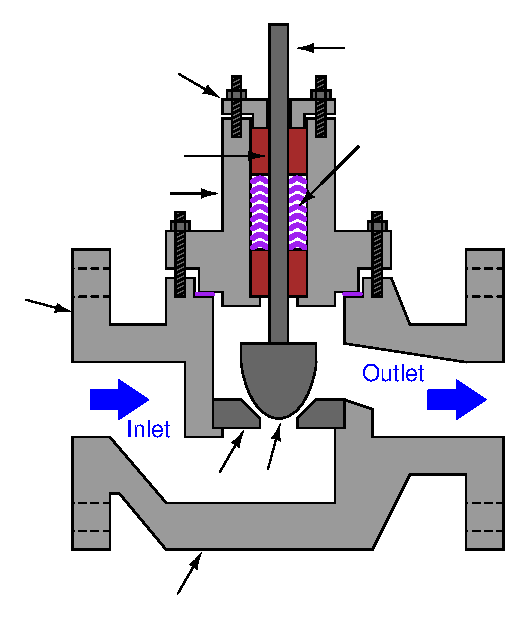
\includegraphics[width=8cm]{i00771x01.eps}$$

Forklar også hvorfor strømningsretningen i figuren går fra venstre mot høyre. Hva ville skjedd om vi i stedet sendte fluidet gjennom denne ventilen fra høyre mot venstre?

\underbar{file i00771}
%(END_QUESTION)





%(BEGIN_ANSWER)

$$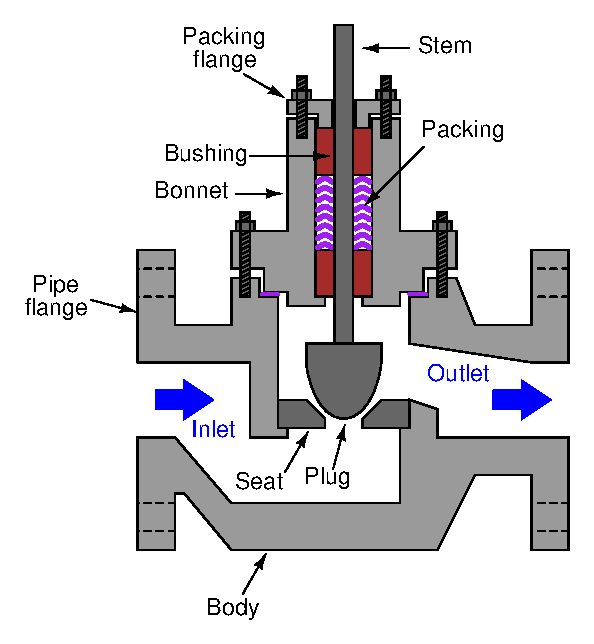
\includegraphics[width=8cm]{i00771x02.eps}$$

Hvis vi brukte denne ventilen «baklengs», ville trykkfallet over pluggen tendere til å «smekke» den igjen når den nærmer seg lukket posisjon. Med andre ord ville prosessfluidets differansetrykk gjøre det svært vanskelig å holde stabil pluggposisjon nær helt lukket.

Dette er faktisk et eksempel på et mekanisk tilbakekoblingssystem. Når ventilen lukkes, øker trykkfallet over den ofte (i mange prosesser) fordi andre trykktap i rørsystemet avtar ved redusert strømning, slik at ventilen blir sittende med det meste av trykkfallet. Siden pluggposisjon påvirker trykkfallet, og trykkfallet gir mekanisk kraft på pluggen, er et tilbakekoblet system i arbeid.

I riktig strømningsretning er tilbakekoblingen negativ: lukking av ventilen gir større trykkfall, som igjen forsøker å holde ventilen åpen. Som ved ekte negativ tilbakekobling virker tilbakekoblingen {\it mot} den opprinnelige handlingen. Jo mer ventilen lukkes, desto mer prøver prosess-trykket å holde den åpen.

I baklengs strømningsretning blir tilbakekoblingen positiv: lukking av ventilen gir større trykkfall, som igjen prøver å lukke ventilen enda mer. Resultatet er tendens til {\it metning} -- ventilen blir stående åpen eller smekker igjen, men unngår stabile mellomstillinger. Dette gjør det svært vanskelig å posisjonere ventilen nær fullt lukket, og gir urolig regulering i nedre del av arbeidsområdet.


%(END_ANSWER)





%(BEGIN_NOTES)


%INDEX% Sluttkontrollelementer, ventil: komponentidentifikasjon i globeventil

%(END_NOTES)


